%• Descrição breve da linguagem X e visão geral da gramática implementada;
%• Descrição de como cada membro da equipe contribuiu no desenvolvimento do trabalho;
%• No final da apresentação, deverá ser demonstrada a execução do software desenvolvido
%usando os arquivos de código fonte sem e com erro sintático (fonte1.txt e fonte3.txt),
%incluindo exibição de parte da árvore sintática para o código sem erro.
%10. Após o encerramento do seminário, o professor pode fazer perguntas a


\documentclass[12pt]{beamer}
\usepackage[utf8]{inputenc}
\usepackage[portuguese]{babel}
\usepackage{graphicx}
\usepackage{colortbl}
\usepackage{color}
\usepackage{breqn}
\usepackage{listings}

\graphicspath{{./images/} {../images/}}
\setbeamertemplate{caption}[numbered]

\definecolor{dkgreen}{rgb}{0,0.6,0}
\definecolor{gray}{rgb}{0.5,0.5,0.5}
\definecolor{mauve}{rgb}{0.58,0,0.82}
\definecolor{laranja_claro}{rgb}{1,0.9,0.5}
\definecolor{laranja_escuro}{rgb}{1,0.5,0.2}
\definecolor{azul_claro}{rgb}{0.5,0.9,1}

\lstset{frame=tb,
    language=C,
    frame=tb,
    aboveskip=3mm,
    belowskip=3mm,
    showstringspaces=false,
    columns=flexible,
    basicstyle={\small\ttfamily},
    numbers=left,
    numberstyle=\tiny\color{gray},
    keywordstyle=\color{blue},
    commentstyle=\color{dkgreen},
    stringstyle=\color{mauve},
    breaklines=true,
    breakatwhitespace=true,
    xleftmargin=.05\textwidth,
    xrightmargin=.05\textwidth,
    tabsize=4,
}

\definecolor{azul}{rgb}{0,0,.5}
\setbeamertemplate{navigation symbols}{}

\usetheme{Frankfurt}
\usecolortheme[named=azul]{structure}

%% Definindo o Autor e o título
\newcommand{\prof}{Newton Spolaôr}
\newcommand{\materia}{Compiladores}

\author[Grupo: c--]{Victor E. Almeida \and Marco A. G. Pedroso}

\title{Analisador sintático e léxico para a linguagem C- -}
\subtitle{Demonstrando o software}
\date{\today}
\institute{UNIOESTE}

\begin{document}
\frame{\titlepage}

\begin{frame}
\frametitle{Conteúdo}
\tableofcontents
\end{frame}

\section{Introdução}\label{Introdução}
\begin{frame}
    \frametitle{Atividades realizadas}
    \begin{itemize}
        \item\textbf{Analisador sintático}: Victor E.;
        \item\textbf{Analisador léxico}: Victor E.;
        \item\textbf{funções auxiliares como log}: Victor E.;
        \item\textbf{Geração da árvore sintática}: Marco G.;
        \item\textbf{Geração dos slides}: Marco G.;
        \item\textbf{Geração do README}: Marco G.;
        \item\textbf{Geração dos arquivos fonte para entrada}: Victor E.;
    \end{itemize}
\end{frame}
\begin{frame}
    \frametitle{Softwares utilizados}
    \begin{itemize}
        \item \textbf{Sistema para compilar}: GNU make 4.3 e gcc 11.2,
        \item \textbf{Linguagem de programação}: C11,
        \item \textbf{Gerador de analisador léxico}: GNU flex 2.6.4;
        \item \textbf{Gerador de analisador sintático}: GNU bison 3.8.2.
    \end{itemize}
\end{frame}


\section{Bison}\label{Bison}
\begin{frame}[t,fragile]{\insertsectionhead}
    \frametitle{Exemplo mínimo do bison}
    \begin{lstlisting}
    %{
        definicoes C
    %}
    %token algum_token
    %start simbolo_inicial

    %%
    simbolo_inicial: algum_token ';'
    %%

    int main() {
        return yyparse();
    }
    \end{lstlisting}
\end{frame}

\begin{frame}[t,fragile]{\insertsectionhead}
    \frametitle{Exemplo de regra do bison}

    \begin{center}
        
    \begin{lstlisting}
    keyword:
	    TOKEN_KEYWORD_IF
	    | TOKEN_KEYWORD_ELSE
	    | TOKEN_KEYWORD_CONST
	    | TOKEN_KEYWORD_FOR
	    | TOKEN_KEYWORD_WHILE
	    | TOKEN_KEYWORD_RETURN
	    | TOKEN_KEYWORD_STRUCT
	    ;
    \end{lstlisting}
    \end{center}
    
\end{frame}

\begin{frame}
    \frametitle{Integrando Flex e bison}
    \begin{figure}[!htb]
        \centering
        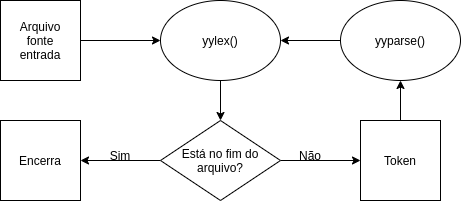
\includegraphics[width=\textwidth]{fluxo}
        \caption{\label{fig:fluxo}Fluxograma do compilador}
    \end{figure}
\end{frame}

\section[Analisador sintático]{Analisador sintático}\label{Analisádor sintático}
\begin{frame}[allowframebreaks]
    \frametitle{Lista de algumas regras gramaticais}
    \begin{itemize}
        \item $<$programa$>$~$::=$ TOKEN\_PREPROCESSOR\_COMMAND $<$programa$>~|$ $<$definition$>~<$programa$>~|~\lambda$
        \item $<$keyword$>::=$ TOKEN\_KEYWORD\_IF $|$ TOKEN\_KEYWORD\_ELSE $|$ TOKEN\_KEYWORD\_CONST $|$\\TOKEN\_KEYWORD\_FOR $|$\\TOKEN\_KEYWORD\_WHILE $|$\\TOKEN\_KEYWORD\_RETURN $|$ TOKEN\_KEYWORD\_STRUCT
        \framebreak
        \item $<$literal$>::=$ TOKEN\_INTEGER\_LITERAL $|$ TOKEN\_FLOAT\_LITERAL $|$ TOKEN\_CHAR\_LITERAL $|$ TOKEN\_STRING\_LITERAL
        \item $<$value $>::=$TOKEN\_ID $|$ TOKEN\_INTEGER\_LITERAL $|$ TOKEN\_FLOAT\_LITERAL
        \item $<$exp$> ::= $ $<$complete\_variable$>~<$exp$>$ $|$ $<$ifel$>~<$exp$>$ $|$ $<$atribuition$>~<$exp$>$ $|$ $<$for$>~<$exp$>$ $|$ $<$while$>~<$exp$>$ $|~\lambda$
    \end{itemize}
\end{frame}

\begin{frame}
    \frametitle{Mão na massa!!}
    \begin{figure}
        \centering
        
\includegraphics[width=.3\textwidth]{pizza.png}
        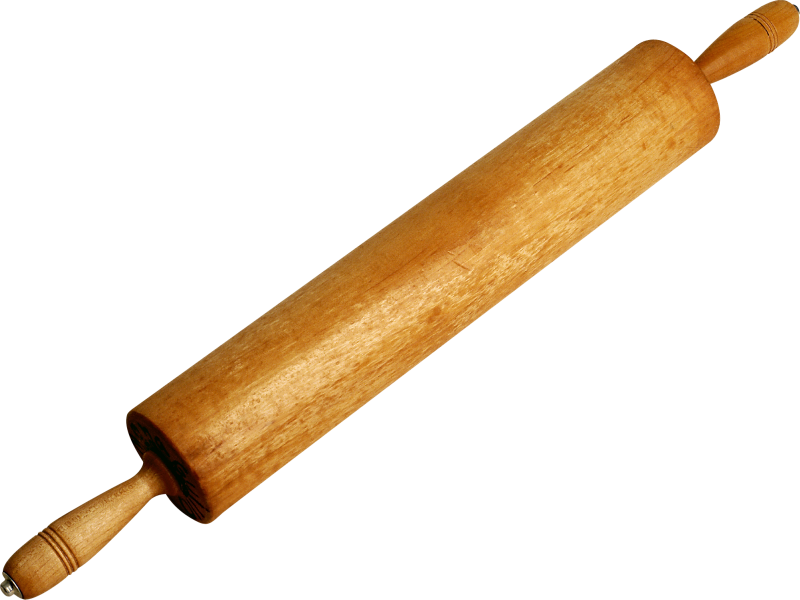
\includegraphics[width=.3\textwidth]{rolo.png}
        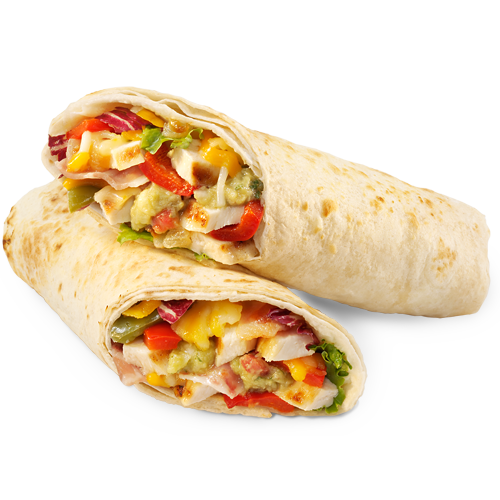
\includegraphics[width=.3\textwidth]{burrito.png}
    \end{figure}
\end{frame}

\section{Conclusão}
\begin{frame}
    \frametitle{Agradecimentos}
    \centering
    \Huge{Perguntas?}
    \begin{figure}
        \centering
        
\includegraphics[width=.3\textwidth]{alerta.png}
        
\includegraphics[width=.3\textwidth]{perigo.png}
        
\includegraphics[width=.3\textwidth]{eletricidade.png}
    \end{figure}
    \Huge{Obrigado pela atenção}
\end{frame}

\end{document}
